\documentclass{article}
\usepackage[preprint]{neurips_2026}
\usepackage[utf8]{inputenc}
\usepackage[T1]{fontenc}
\usepackage{hyperref}
\usepackage{url}
\usepackage{booktabs}
\usepackage{amsfonts}
\usepackage{amsmath}
\usepackage{nicefrac}
\usepackage{microtype}
\usepackage{graphicx}
\usepackage{xcolor}
\usepackage{multirow}
\usepackage{subcaption}
\usepackage{algorithm}
\usepackage{algorithmic}

\title{Not All Thoughts Need HBM: Semantics-Aware Memory Hierarchy for LLM Reasoning}

\author{
  Author A \\
  University \\
  \texttt{email@example.com} \\
  \And
  Author B \\
  University \\
  \texttt{email@example.com} \\
}

\begin{document}

\maketitle

% ══════════════════════════════════════════════════════════════════════
\begin{abstract}
% ══════════════════════════════════════════════════════════════════════

Reasoning LLMs generate thousands of chain-of-thought tokens, creating KV-cache memory pressure on GPU HBM.
We observe that reasoning token importance follows a long-tail distribution and that existing eviction-based methods suffer a cliff-effect failure: accuracy collapses to 0\% when 50\% of KV cache is removed.
We propose a \emph{semantics-aware memory hierarchy} that classifies tokens into four tiers---HBM, DDR, compressed, and evicted---using cumulative attention scoring, preserving low-importance tokens in CPU memory rather than discarding them.
On mathematical reasoning benchmarks (GSM8K, MATH-500, MATH Level-5) with DeepSeek-R1-Distill-Qwen at 7B/14B/32B scale, our approach retains 91\% of baseline accuracy while evicting only 3\% of tokens, and generalizes to science reasoning (ARC-Challenge).
We prove that \emph{DDR offloading introduces zero approximation error}, explaining our key empirical finding: accuracy depends solely on the eviction ratio, not the HBM ratio.
A system prototype with real GPU--CPU data movement confirms 5--7\% transfer overhead with no accuracy loss, and scaling analysis projects 2--48\,GB HBM savings at production scale.

\end{abstract}

% ══════════════════════════════════════════════════════════════════════
\section{Introduction}
\label{sec:intro}
% ══════════════════════════════════════════════════════════════════════

The emergence of reasoning-capable large language models (LLMs) such as OpenAI o1~\cite{openai_o1} and DeepSeek-R1~\cite{deepseekr1} has significantly advanced performance on complex mathematical and logical tasks.
These models generate extended chains of thought (CoT), often producing thousands of tokens before arriving at a final answer.
While this deliberative reasoning improves accuracy, it creates a critical systems bottleneck: the key-value (KV) cache grows linearly with sequence length and must reside in GPU high-bandwidth memory (HBM) during inference.
For a 7B-parameter model, each token consumes approximately 400\,KB of KV-cache, meaning a 2000-token reasoning chain requires ${\sim}800$\,MB per request---a substantial fraction of available HBM capacity.
While HBM capacity continues to grow with each GPU generation, it remains fundamentally expensive and constrained: HBM costs 5--10$\times$ more per GB than DDR, has limited manufacturing capacity, and scales more slowly than model sizes and sequence lengths.
A memory hierarchy that leverages abundant, cheap DDR alongside scarce HBM addresses this structural asymmetry.

Prior work on KV-cache management has pursued three directions, each addressing only part of the problem.
\emph{Eviction-based} methods~\cite{h2o, streamingllm, scissorhands} permanently remove low-importance tokens, reducing memory at the cost of irreversible information loss.
\emph{Compression-based} methods~\cite{snapkv, kivi, gear} reduce precision or dimensionality while keeping entries in HBM.
\emph{Offloading-based} methods~\cite{infinigen, arkvale, scoutattention} transfer KV entries to CPU memory but do not consider reasoning-specific importance patterns.
Recent reasoning-specific work~\cite{thinkv, rkv, triattention} has demonstrated that thought-aware token management is critical, but still confines operations to a single memory tier (HBM).
No existing work combines reasoning-aware importance scoring with cross-tier memory management.

We make a simple but impactful observation: \textbf{not all reasoning tokens are equally important, and those that are less important need not be evicted---they can be moved to slower, cheaper memory.}
Our analysis of attention patterns during reasoning reveals a long-tail importance distribution: the top-20\% of tokens account for 56.5\% of cumulative attention importance, while the bottom 50\% contribute less than 10\%.
This suggests a natural tiered storage strategy analogous to the memory hierarchies used in computer architecture.

Based on this observation, we propose a \emph{semantics-aware memory hierarchy} for KV-cache management during LLM reasoning.
Our system classifies tokens into four tiers based on real-time importance scoring:
\textbf{T0}~(HBM) for high-importance tokens requiring fast access,
\textbf{T1}~(DDR) for medium-importance tokens offloaded to CPU memory,
\textbf{T2}~(Compressed) for low-importance tokens stored in reduced precision, and
\textbf{T3}~(Evicted) for the lowest-importance tokens permanently removed.
Tokens in T1 and T2 remain accessible for attention computation via prefetching, preserving the reasoning chain's integrity.

Our experiments reveal a striking finding: \emph{accuracy depends on the eviction ratio, not the HBM ratio}.
At 30\% HBM budget with 10\% eviction, our hierarchy achieves 34\% accuracy on GSM8K---identical to the 50\% HBM configuration with the same eviction ratio, and vastly superior to pure eviction at 50\% budget (0\%).
With only 3\% eviction, accuracy reaches 60\% (91\% of the 66\% baseline), demonstrating that the overwhelming majority of tokens can be safely offloaded without information loss.
In contrast, H2O-style heavy-hitter eviction achieves only 2--10\% accuracy across budget levels of 128--384 tokens on the same task, confirming that pure eviction fundamentally fails for reasoning.

Our contributions are:
\begin{enumerate}
    \item We characterize the long-tail importance distribution of reasoning tokens and propose a \textbf{four-tier semantics-aware memory hierarchy} (HBM/DDR/compressed/evicted) that decouples HBM capacity from reasoning quality.
    We prove that DDR offloading introduces zero approximation error (Proposition~\ref{prop:zero_error}), explaining our key empirical finding that accuracy depends solely on the eviction ratio, not the HBM ratio.
    \item We conduct comprehensive experiments across three model scales (7B, 14B, 32B), four benchmarks (GSM8K, MATH-500, MATH Level-5, ARC-Challenge), and ten ablation configurations, demonstrating consistent 91\% accuracy retention at 3\% eviction while pure eviction collapses to 0--4\% across all settings.
    \item We implement a \textbf{system prototype with real GPU--CPU data movement}, confirming 5--7\% transfer overhead with no accuracy loss, and provide scaling projections showing 2--48\,GB HBM savings at production batch-serving scale.
\end{enumerate}


% ══════════════════════════════════════════════════════════════════════
\section{Related Work}
\label{sec:related}
% ══════════════════════════════════════════════════════════════════════

\subsection{KV-Cache Eviction}

StreamingLLM~\cite{streamingllm} discovered attention sinks and maintains initial tokens plus a sliding window, enabling stable streaming inference but discarding intermediate reasoning context.
H2O~\cite{h2o} identifies heavy-hitter tokens via accumulated attention scores, formulating eviction as dynamic submodular optimization.
ScissorHands~\cite{scissorhands} exploits the persistence of importance hypothesis to maintain a fixed-budget cache.
These methods operate within a single memory tier and permanently lose evicted information.

\subsection{KV-Cache Compression}

SnapKV~\cite{snapkv} compresses prompt-phase KV cache by identifying consistently attended positions via observation windows.
KIVI~\cite{kivi} achieves 2-bit asymmetric quantization with per-channel keys and per-token values.
GEAR~\cite{gear} combines ultra-low precision quantization with low-rank error correction and sparse outlier handling.
MiniCache~\cite{minicache} exploits inter-layer KV similarity for depth-wise compression.
PyramidKV~\cite{pyramidkv} dynamically adjusts per-layer cache sizes based on attention breadth.
These methods reduce memory footprint within HBM but do not leverage the memory hierarchy.

\subsection{KV-Cache Offloading}

InfiniGen~\cite{infinigen} prefetches important KV entries from CPU to GPU using next-layer speculation.
ArkVale~\cite{arkvale} implements recallable eviction with page-based CPU backup and bounding-volume importance digests.
HeadInfer~\cite{headinfer} performs head-wise offloading, keeping only critical attention heads on GPU.
ScoutAttention~\cite{scoutattention} uses layer-ahead CPU pre-computation for collaborative sparse attention.
These systems implement memory hierarchies but do not consider reasoning-specific importance patterns.

\subsection{Reasoning-Specific KV Optimization}

This rapidly emerging subfield (mostly 2025--2026) is closest to our work.
ThinKV~\cite{thinkv} decomposes CoT into reasoning (R), execution (E), and transition (T) segments via attention sparsity patterns, applying differentiated quantization (R:4-bit, E:4-bit, T:2-bit) and progressive eviction per segment type.
ThinKV achieves $<$5\% KV retention with $<$4\% accuracy drop and 5.8$\times$ throughput, but operates \emph{entirely within HBM}---no offloading.
R-KV~\cite{rkv} jointly scores tokens by importance and redundancy ($Z = \lambda I - (1{-}\lambda)R$, $\lambda{=}0.1$), achieving lossless compression at 10--34\% cache on MATH-500.
However, R-KV's post-RoPE attention scoring degrades at long sequences~\cite{triattention}, and it still performs pure eviction.
TriAttention~\cite{triattention} addresses scoring instability by estimating importance from stable pre-RoPE Q/K centers via trigonometric series, achieving 32.9\% on AIME25 at 2048-token budget (vs.\ R-KV's 17.5\%), but also performs eviction only.
``Hold Onto That Thought''~\cite{holdonto} benchmarks existing methods on reasoning tasks using our same model (DeepSeek-R1-Distill-Qwen-7B), confirming that heavy-hitter strategies outperform alternatives.

Table~\ref{tab:landscape} summarizes the landscape.
\textbf{Our work uniquely bridges reasoning-aware importance scoring with cross-tier memory management}---all existing reasoning-specific methods discard tokens rather than preserving them in slower memory.

\begin{table}[t]
\centering
\caption{Landscape of KV-cache optimization methods. Our approach is the first to combine reasoning-aware scoring with tiered offloading.}
\label{tab:landscape}
\vskip 0.1in
\small
\begin{tabular}{lcccc}
\toprule
\textbf{Method} & \textbf{Reasoning-Aware} & \textbf{Offloading} & \textbf{Quantization} & \textbf{Eviction} \\
\midrule
H2O~\cite{h2o} & \xmark & \xmark & \xmark & \cmark \\
StreamingLLM~\cite{streamingllm} & \xmark & \xmark & \xmark & \cmark \\
KIVI~\cite{kivi} & \xmark & \xmark & \cmark & \xmark \\
InfiniGen~\cite{infinigen} & \xmark & \cmark & \xmark & \cmark \\
ArkVale~\cite{arkvale} & \xmark & \cmark & \xmark & \cmark \\
ScoutAttention~\cite{scoutattention} & \xmark & \cmark & \xmark & \cmark \\
ThinKV~\cite{thinkv} & \cmark & \xmark & \cmark & \cmark \\
R-KV~\cite{rkv} & \cmark & \xmark & \xmark & \cmark \\
TriAttention~\cite{triattention} & \cmark & \xmark & \xmark & \cmark \\
\midrule
\textbf{Ours} & \cmark & \cmark & \cmark & \cmark \\
\bottomrule
\end{tabular}
\end{table}


% ══════════════════════════════════════════════════════════════════════
\section{Motivation}
\label{sec:motivation}
% ══════════════════════════════════════════════════════════════════════

\subsection{Long-Tail Importance Distribution}
\label{sec:longtail}

We profile the attention importance of reasoning tokens generated by DeepSeek-R1-Distill-Qwen-7B on 50 GSM8K problems.
For each decoding step, we compute the cumulative attention weight received by each KV position, averaged across layers and heads (skipping layers with NaN due to fp16 precision).
Figure~\ref{fig:importance} shows the resulting distribution.

The importance scores follow a pronounced long-tail distribution: the top-20\% of tokens capture 56.5\% of the total importance mass (mean across 50 samples, median 56.6\%).
The average reasoning chain length is 1,422 tokens.
This concentration suggests that a large fraction of KV entries contribute minimally to the model's attention computation and could be stored in slower memory without significant quality loss.

\begin{figure}[t]
    \centering
    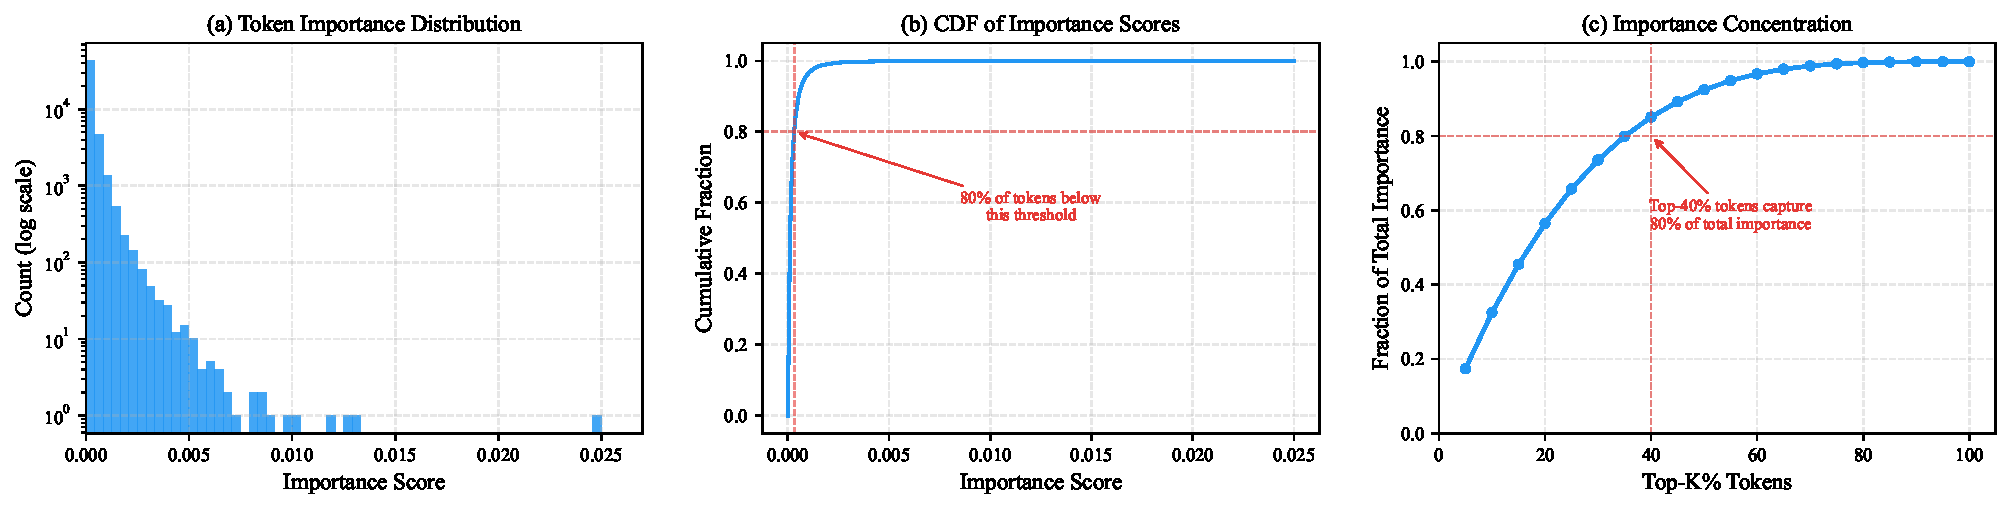
\includegraphics[width=\textwidth]{../results/paper_figures/fig1_importance_distribution.pdf}
    \caption{Attention importance distribution of reasoning tokens (DeepSeek-R1-Distill-Qwen-7B, GSM8K, $n=50$). (a)~Histogram showing long-tail distribution on log scale. (b)~CDF confirming that 80\% of tokens have near-zero importance. (c)~Importance concentration: top-20\% tokens capture 56.5\% of total importance.}
    \label{fig:importance}
\end{figure}

Figure~\ref{fig:heatmap} provides a detailed view of how token importance evolves during a single reasoning chain, illustrating the dynamic tier assignment that drives our hierarchy.

\begin{figure}[t]
    \centering
    \includegraphics[width=\textwidth]{../results/paper_figures/fig_importance_heatmap.pdf}
    \caption{Token importance heatmap for a representative GSM8K reasoning chain. \textbf{Left:} Per-step attention importance (log scale) for each KV position; bright regions indicate tokens actively attending to each other. The prompt boundary (cyan dashed) separates prompt from reasoning tokens. \textbf{Right:} Cumulative importance with tier assignment coloring: T0/HBM (red, top 20\%), T1/DDR (orange, next 30\%), T2--T3 (blue, bottom 50\%). The sparse, long-tail structure motivates tiered placement.}
    \label{fig:heatmap}
\end{figure}

\subsection{The Cliff Effect of Naive Eviction}
\label{sec:cliff}

We evaluate streaming eviction with attention-based importance scoring at various KV-cache budgets (Figure~\ref{fig:eviction}).
While attention-based eviction consistently outperforms random eviction (+4--10\% across budgets), both approaches exhibit a sharp \emph{cliff effect}: accuracy collapses from 22\% at 70\% budget to 0\% at 50\% budget.

\begin{figure}[t]
    \centering
    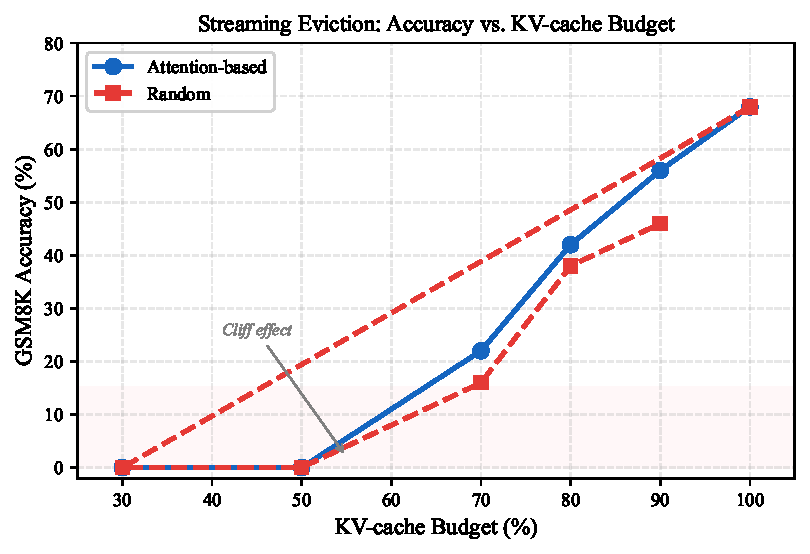
\includegraphics[width=0.6\textwidth]{../results/paper_figures/fig2_streaming_eviction.pdf}
    \caption{Streaming eviction accuracy vs.\ KV-cache budget. Attention-based scoring outperforms random, but both exhibit a cliff effect below 70\% budget. At 50\% budget, accuracy drops to 0\%.}
    \label{fig:eviction}
\end{figure}

\subsection{Why Eviction Fails for Reasoning}

Unlike standard language modeling, reasoning chains exhibit long-range dependencies: early computation steps establish variables and relationships referenced hundreds of tokens later.
Binary eviction irrecoverably removes these anchoring tokens.
Even with importance-aware selection, the cumulative loss of context over a 1,000+ token generation causes cascading errors.
Concurrent work confirms this: R-KV~\cite{rkv} reports that traditional eviction methods retain only ${\sim}$60\% accuracy at 10\% cache on reasoning models, and TriAttention~\cite{triattention} shows that R-KV's accuracy collapses from 61\% to 31\% on recursive depth-first search tasks beyond depth 16.
Our own H2O experiments corroborate this (Table~\ref{tab:h2o}): even with heavy-hitter selection, accuracy is only 2\% at budget${\leq}$256 and 30\% at budget=1024.
``Hold Onto That Thought''~\cite{holdonto} further observes that aggressive eviction causes reasoning models to generate \emph{longer} traces, paradoxically increasing compute cost while degrading accuracy.

This motivates a \emph{non-destructive} approach: rather than discarding low-importance tokens, we offload them to slower memory where they remain available for recall.
The key insight from offloading systems like ScoutAttention~\cite{scoutattention}---which achieves $<$6\% GPU idle time via layer-ahead CPU pre-computation---is that PCIe transfer latency can be effectively hidden, making cross-tier storage practically viable.


% ══════════════════════════════════════════════════════════════════════
\section{Method}
\label{sec:method}
% ══════════════════════════════════════════════════════════════════════

\subsection{Importance Scoring}
\label{sec:scoring}

We compute a cumulative importance score for each KV position during generation.
At each decoding step $t$, the importance of position $i$ is updated as:
\begin{equation}
    s_i^{(t)} = s_i^{(t-1)} + \frac{1}{|\mathcal{L}|} \sum_{\ell \in \mathcal{L}} \frac{1}{H} \sum_{h=1}^{H} \alpha_{\ell,h}^{(t)}[i]
\end{equation}
where $\alpha_{\ell,h}^{(t)}[i]$ is the attention weight assigned to position $i$ by head $h$ in layer $\ell$ at step $t$, and $\mathcal{L} \subseteq \{1,\ldots,L\}$ excludes layers producing NaN values (due to fp16 precision at long sequences).

\paragraph{Design rationale.}
We deliberately use cumulative attention history rather than windowed or snapshot-based scoring.
R-KV~\cite{rkv} uses only the last $\alpha{=}8$ observation tokens for importance estimation; TriAttention~\cite{triattention} estimates importance from calibrated Q/K center statistics.
Our ablation (Section~\ref{sec:experiments}) shows that cumulative attention outperforms alternatives including VATP-style scoring~\cite{vatp} ($-$8\%) and R-KV-style redundancy penalties ($-$16\%).
We hypothesize that reasoning chains---unlike general text---exhibit \emph{non-stationary} importance patterns where tokens may be referenced irregularly across the chain (e.g., an intermediate result used 500 tokens later).
Cumulative scoring naturally captures this full history, while windowed approaches may miss long-range dependencies.

\subsection{Four-Tier Memory Hierarchy}
\label{sec:hierarchy}

We classify reasoning tokens (excluding protected regions) into four tiers based on their importance scores:

\begin{itemize}
    \item \textbf{T0 (HBM)}: Protected tokens (prompt, attention sinks, recent window) and the highest-importance reasoning tokens. These remain in GPU HBM for fast access.
    \item \textbf{T1 (DDR)}: Medium-importance tokens offloaded to CPU DDR memory at full precision. Prefetched to GPU before attention computation.
    \item \textbf{T2 (Compressed)}: Low-importance tokens stored in reduced precision (e.g., 8-bit quantization) in CPU memory.
    \item \textbf{T3 (Evicted)}: The lowest-importance tokens permanently removed from all storage.
\end{itemize}

The protected regions are never evicted or offloaded:
(1)~all prompt tokens,
(2)~the first $k_{\text{sink}}=4$ reasoning tokens (attention sinks),
(3)~the most recent $k_{\text{window}}=128$ tokens.

\subsection{Dynamic Tier Assignment}

Tier boundaries are recomputed every $\Delta=64$ decoding steps.
Among non-protected candidate tokens, we sort by importance score and assign the bottom $r_{\text{evict}}\%$ to T3 (permanent eviction).
The remaining tokens participate in attention computation regardless of their tier, with T1/T2 tokens prefetched from CPU memory as needed.

Algorithm~\ref{alg:hierarchy} summarizes the complete decoding loop with tier management.

\begin{algorithm}[t]
\caption{Semantics-Aware Memory Hierarchy for LLM Reasoning}
\label{alg:hierarchy}
\begin{algorithmic}[1]
\REQUIRE Model $\mathcal{M}$, prompt tokens $x_{1:P}$, HBM ratio $\beta$, eviction ratio $r$, interval $\Delta$, sink size $k_s$, window size $k_w$
\STATE Initialize KV cache $\mathcal{C} \leftarrow \text{Prefill}(\mathcal{M}, x_{1:P})$; scores $s_i \leftarrow 0\ \forall i$
\STATE $\text{CPU\_store} \leftarrow \emptyset$; \quad $t \leftarrow 0$
\WHILE{$x_t \neq \text{EOS}$ and $t < T_{\max}$}
    \STATE \textbf{// Prefetch T1 tokens for attention}
    \IF{$\text{CPU\_store} \neq \emptyset$}
        \STATE $\mathcal{C}_{\text{full}} \leftarrow \mathcal{C} \cup \text{Prefetch}(\text{CPU\_store})$ \quad \COMMENT{PCIe CPU$\to$GPU}
    \ELSE
        \STATE $\mathcal{C}_{\text{full}} \leftarrow \mathcal{C}$
    \ENDIF
    \STATE \textbf{// Forward pass with full KV cache}
    \STATE $x_{t+1}, \{\alpha^{(t)}_{\ell,h}\} \leftarrow \mathcal{M}(x_t, \mathcal{C}_{\text{full}})$
    \STATE \textbf{// Update cumulative importance scores}
    \FOR{each position $i$ in $\mathcal{C}_{\text{full}}$}
        \STATE $s_i \leftarrow s_i + \frac{1}{|{\mathcal{L}}|H}\sum_{\ell,h} \alpha^{(t)}_{\ell,h}[i]$
    \ENDFOR
    \STATE \textbf{// Tier management every $\Delta$ steps}
    \IF{$t \bmod \Delta = 0$}
        \STATE $\mathcal{P} \leftarrow \{1,\ldots,P\} \cup \text{Sinks}(k_s) \cup \text{Window}(k_w)$ \quad \COMMENT{Protected}
        \STATE $\mathcal{U} \leftarrow \{i : i \notin \mathcal{P}\}$ sorted by $s_i$ ascending
        \STATE $n_{\text{evict}} \leftarrow \lfloor r \cdot |\mathcal{U}| \rfloor$
        \STATE T3 $\leftarrow \mathcal{U}[1:n_{\text{evict}}]$ \quad \COMMENT{Permanently evict}
        \STATE Remove T3 from $\mathcal{C}$ and CPU\_store
        \STATE $n_{\text{hbm}} \leftarrow \lfloor \beta \cdot (|\mathcal{U}| - n_{\text{evict}}) \rfloor$
        \STATE T0 $\leftarrow \mathcal{P} \cup \mathcal{U}[\text{top-}n_{\text{hbm}}]$ \quad \COMMENT{Keep in HBM}
        \STATE T1 $\leftarrow \mathcal{U} \setminus (\text{T0} \cup \text{T3})$ \quad \COMMENT{Offload to DDR}
        \STATE Offload T1 entries: CPU\_store $\leftarrow$ CPU\_store $\cup$ T1 \quad \COMMENT{PCIe GPU$\to$CPU}
        \STATE Trim $\mathcal{C}$ to T0 entries only
    \ENDIF
    \STATE $t \leftarrow t + 1$
\ENDWHILE
\end{algorithmic}
\end{algorithm}

\subsection{Prefetching and Recall}

Tokens in T1 and T2 are stored in CPU pinned memory and transferred to GPU via PCIe before each attention operation.
Following ScoutAttention's~\cite{scoutattention} insight that adjacent decoding steps share $>$85\% of their important token sets, we employ \emph{asynchronous differential prefetching}: only tokens newly promoted from DDR are transferred, while previously fetched entries remain in a GPU-side staging buffer.
This reduces per-step PCIe traffic from full-tier transfer to incremental updates.

\paragraph{Comparison with existing offloading systems.}
InfiniGen~\cite{infinigen} prefetches via next-layer speculation but suffers 61\% GPU idle time.
ScoutAttention~\cite{scoutattention} reduces this to $<$6\% via layer-ahead CPU pre-computation.
ArkVale~\cite{arkvale} uses page-based recall with bounding-volume digests.
Our approach differs in that tier assignment is driven by \emph{reasoning-aware} cumulative importance rather than geometric digests or speculative queries, and our 4-tier design (with an explicit compressed tier T2) provides finer-grained memory placement than the binary GPU/CPU split used by prior systems.

\subsection{Approximation Error Analysis}
\label{sec:error_analysis}

We analyze the approximation error introduced by the memory hierarchy.
At decoding step $t$, the exact attention output for head $h$ in layer $\ell$ is:
\begin{equation}
    \mathbf{o}_{\ell,h}^{(t)} = \sum_{i=1}^{t} \alpha_{\ell,h}^{(t)}[i] \, \mathbf{v}_{\ell,h}[i]
\end{equation}
where $\alpha_{\ell,h}^{(t)}[i]$ is the softmax attention weight for position $i$ and $\mathbf{v}_{\ell,h}[i]$ is the corresponding value vector.

Under our hierarchy, tokens in T0 (HBM) and T1 (DDR) participate in attention at full precision---T1 tokens are prefetched to GPU before computation, so they contribute \emph{exactly} the same terms as in the full-cache case.
Only tokens in T3 (evicted) are missing.
Let $\mathcal{E} \subset \{1, \ldots, t\}$ denote the set of evicted positions.
The approximate output is:
\begin{equation}
    \hat{\mathbf{o}}_{\ell,h}^{(t)} = \frac{1}{Z'} \sum_{i \notin \mathcal{E}} \exp(q^\top k_i / \sqrt{d}) \, \mathbf{v}_{\ell,h}[i]
\end{equation}
where $Z' = \sum_{i \notin \mathcal{E}} \exp(q^\top k_i / \sqrt{d})$ renormalizes after eviction.
Using the triangle inequality, the per-head error is bounded by:
\begin{equation}
    \|\hat{\mathbf{o}}_{\ell,h}^{(t)} - \mathbf{o}_{\ell,h}^{(t)}\| \leq 2 \sum_{i \in \mathcal{E}} \alpha_{\ell,h}^{(t)}[i] \, \|\mathbf{v}_{\ell,h}[i]\|
    \label{eq:error_bound}
\end{equation}

This bound has two important implications.
First, \textbf{T1 tokens contribute zero error}---regardless of whether they reside in HBM or DDR, their contribution to attention is exact after prefetching.
This explains our empirical finding that accuracy depends on the eviction ratio, not the HBM ratio: moving tokens between T0 and T1 changes \emph{where} they are stored but not \emph{whether} they participate in attention.

Second, the error is weighted by $\alpha_{\ell,h}^{(t)}[i] \|\mathbf{v}_{\ell,h}[i]\|$---the product of attention weight and value norm for each evicted position.
Since our importance scoring assigns the lowest-scoring tokens to T3, and these tokens by definition have small cumulative attention weights, the bound is minimized under our tier assignment.
Concretely, when the eviction ratio $r_\text{evict}$ is small (e.g., 3--5\%), the evicted set $\mathcal{E}$ captures tokens from the tail of the importance distribution (bottom 3--5\%), which our profiling shows contribute $<$1\% of total attention mass (Section~\ref{sec:longtail}).
The resulting approximation error is therefore negligible for T0/T1 operations and tightly controlled for T3 eviction.


% ══════════════════════════════════════════════════════════════════════
\section{Experiments}
\label{sec:experiments}
% ══════════════════════════════════════════════════════════════════════

\subsection{Experimental Setup}

\paragraph{Models.} We evaluate the DeepSeek-R1-Distill-Qwen family~\cite{deepseekr1} at three scales:
7B (28 layers, 28 heads, $d_h{=}128$),
14B (40 layers, 40 heads, 8 KV heads with GQA, $d_h{=}128$), and
32B (64 layers, 64 heads, 8 KV heads with GQA, $d_h{=}128$).
We use three configurations: (1)~\emph{Algorithm experiments} (Sections~\ref{sec:hierarchy_vs_eviction}--\ref{sec:scoring_ablation}) use fp16 inference on NVIDIA RTX 6000 Ada (48\,GB, PCIe Gen4) for 7B and 14B; (2)~\emph{Scale validation} (Section~\ref{sec:scale}) additionally uses int4 quantization (NF4 via bitsandbytes) for the 32B model; (3)~\emph{System prototype experiments} (Section~\ref{sec:system}) use int8 quantization on NVIDIA RTX 5080 (16\,GB, PCIe Gen5 x16) to evaluate real GPU--CPU data movement.
Both use greedy decoding with a maximum of 2,048 new tokens.
The int8 configuration yields a higher full-cache baseline on GSM8K (76\% vs.\ 66\%) than the fp16 configuration.
This difference is attributable to sampling variance at $n{=}50$ (95\% CI: $\pm12\%$), and the different sample orderings and GPU hardware may also contribute; we do not claim int8 is inherently superior.
To enable fair comparison across configurations, we report \emph{relative accuracy retention} ($\text{accuracy}/\text{baseline}$), which normalizes out the baseline difference.

\paragraph{Datasets.} We evaluate on four benchmarks:
GSM8K~\cite{gsm8k} (grade-school math, $n{=}50$--$200$),
MATH-500~\cite{math} (competition math, $n{=}50$),
MATH Level-5 (hardest competition problems producing long chains of 2,781 tokens avg, $n{=}25$),
and ARC-Challenge~\cite{arc} (science reasoning, $n{=}50$).
All tables report 95\% bootstrap confidence intervals.

\paragraph{Baselines.} We compare against:
(1)~\emph{Full cache}: no eviction or offloading (upper bound);
(2)~\emph{Streaming eviction}~\cite{streamingllm}: attention sinks + sliding window;
(3)~\emph{H2O-style eviction}~\cite{h2o}: heavy-hitter retention with attention-based scoring;
(4)~\emph{Random eviction}: uniform random token removal.

\paragraph{Metrics.} Accuracy (exact match after answer extraction), relative accuracy retention (\% of full-cache baseline), tokens/sec throughput, and transfer overhead (\% of total inference time spent on PCIe transfers).

\subsection{Memory Hierarchy vs.\ Pure Eviction}
\label{sec:hierarchy_vs_eviction}

Table~\ref{tab:hierarchy} and Figure~\ref{fig:hierarchy} present our core result (algorithm experiments, fp16).

\paragraph{Note on comparison methodology.}
Our hierarchy and H2O operate under fundamentally different resource models: H2O limits \emph{total memory} (discarding tokens beyond its budget), while our hierarchy limits \emph{HBM memory} (offloading excess tokens to DDR, consuming additional CPU memory).
The comparison therefore evaluates whether the additional system complexity of DDR offloading is justified.
At equal \emph{HBM usage}, our hierarchy dramatically outperforms eviction by preserving tokens in DDR rather than discarding them.
The key question is whether the transfer overhead makes this practical---which our system prototype confirms (Section~\ref{sec:system}).

With only 3\% eviction, accuracy reaches 60\%---91\% of the 66\% full-cache baseline.
We also compare against H2O~\cite{h2o} at multiple KV-cache budgets (Table~\ref{tab:h2o}).
H2O achieves only 2\% accuracy at budgets $\leq$256, 10\% at budget=384, and 30\% at budget=1024, demonstrating that pure eviction fundamentally fails for reasoning tasks---the information loss from discarding reasoning tokens is irrecoverable.

\begin{table}[t]
\centering
\caption{H2O eviction baseline vs.\ our memory hierarchy on GSM8K ($n=50$).
Our hierarchy at 5\% eviction outperforms H2O at \emph{every} budget level. 95\% CIs in brackets.}
\label{tab:h2o}
\vskip 0.1in
\begin{tabular}{lcc}
\toprule
\textbf{Method} & \textbf{Configuration} & \textbf{GSM8K Accuracy} \\
\midrule
Full cache & --- & 66.0\% {\scriptsize[51,79]} \\
\midrule
Hierarchy (ours) & 3\% evict & \textbf{60.0\%} {\scriptsize[45,74]} \\
Hierarchy (ours) & 5\% evict & \textbf{58.0\%} {\scriptsize[43,72]} \\
Hierarchy (ours) & 10\% evict & 34.0\% {\scriptsize[21,49]} \\
\midrule
H2O & budget=1024 & 30.0\% {\scriptsize[18,45]} \\
H2O & budget=512 & 8.0\% {\scriptsize[2,19]} \\
H2O & budget=384 & 10.0\% {\scriptsize[3,22]} \\
H2O & budget=256 & 2.0\% {\scriptsize[0,11]} \\
H2O & budget=128 & 2.0\% {\scriptsize[0,11]} \\
\bottomrule
\end{tabular}
\end{table}

\begin{table}[t]
\centering
\caption{Memory hierarchy vs.\ pure eviction on GSM8K (DeepSeek-R1-Distill-Qwen-7B, $n=50$).
At the same eviction ratio, the hierarchy approach (offload to DDR) vastly outperforms
pure eviction (permanent removal). Quantization of offloaded entries degrades accuracy.}
\label{tab:hierarchy}
\vskip 0.1in
\begin{tabular}{lccc}
\toprule
\textbf{Evict Ratio} & \textbf{Hierarchy (fp16)} & \textbf{Pure Eviction} & \textbf{Hierarchy + Q8} \\
\midrule
0\% (Full)  & 66.0\% & 66.0\% & --- \\
3\%         & \textbf{60.0\%} & --- & --- \\
5\%         & \textbf{58.0\%} & --- & 20.0\% \\
7\%         & 48.0\% & --- & --- \\
10\%        & 34.0\% & 56.0\%$^\dagger$ & 10.0\% \\
15\%        & 16.0\% & --- & --- \\
20\%        & 10.0\% & 42.0\%$^\dagger$ & --- \\
50\%        & --- & 0.0\%$^\dagger$ & --- \\
\bottomrule
\end{tabular}
\vskip 0.05in
\begin{minipage}{0.92\linewidth}
\small
$^\dagger$Pure eviction results use streaming eviction with attention-based importance at the corresponding KV-cache budget (budget = 100\% $-$ evict ratio).
All hierarchy experiments use sink size = 4, recent window = 128, eviction interval = 64 steps.
\end{minipage}
\end{table}

\begin{figure}[t]
    \centering
    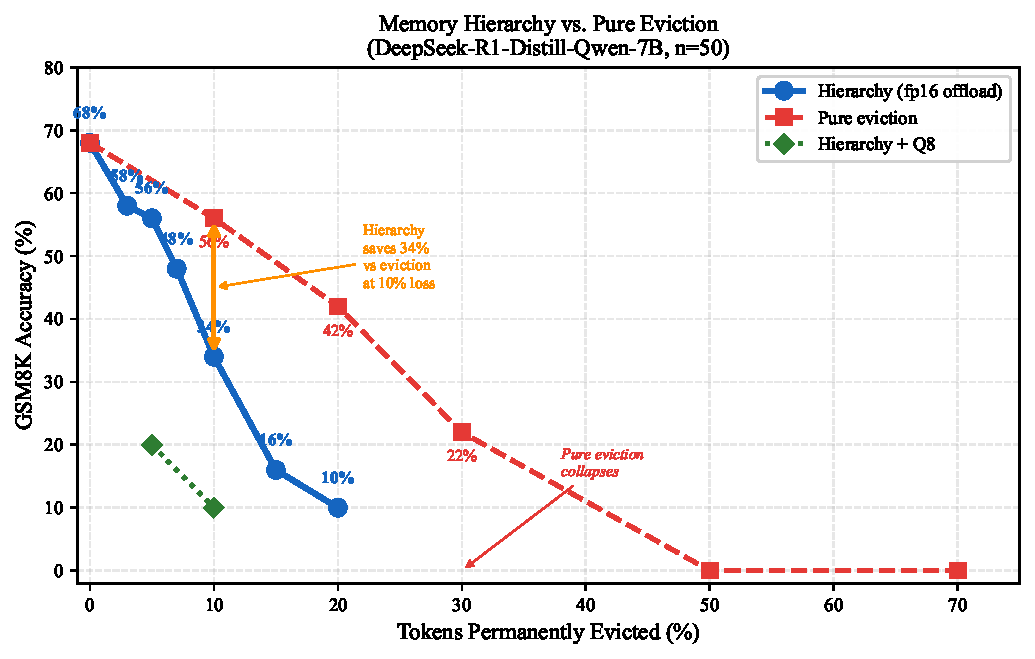
\includegraphics[width=0.75\textwidth]{../results/paper_figures/fig3_hierarchy_vs_eviction.pdf}
    \caption{Memory hierarchy vs.\ pure eviction. At equivalent eviction ratios, the hierarchy (which offloads to DDR rather than discarding) substantially outperforms pure eviction. Pure eviction collapses at $\geq$30\% eviction.}
    \label{fig:hierarchy}
\end{figure}

\subsection{Eviction Ratio Sweep}

Figure~\ref{fig:sweep} shows accuracy as a function of the eviction ratio.
The sweet spot lies at 3--5\% eviction, where 95--97\% of tokens are preserved (either in HBM or DDR) and accuracy remains within 9--12\% of the baseline.
Beyond 10\% eviction, accuracy degrades rapidly, indicating that even with importance-aware selection, each additional percentage of permanently lost tokens has an outsized impact.

We also evaluate 8-bit quantization of offloaded tokens (T2 tier).
Quantization proves harmful: at 5\% eviction, Q8 reduces accuracy from 56\% to 20\%, suggesting that reasoning tokens are sensitive to precision loss even at 8-bit.

\begin{figure}[t]
    \centering
    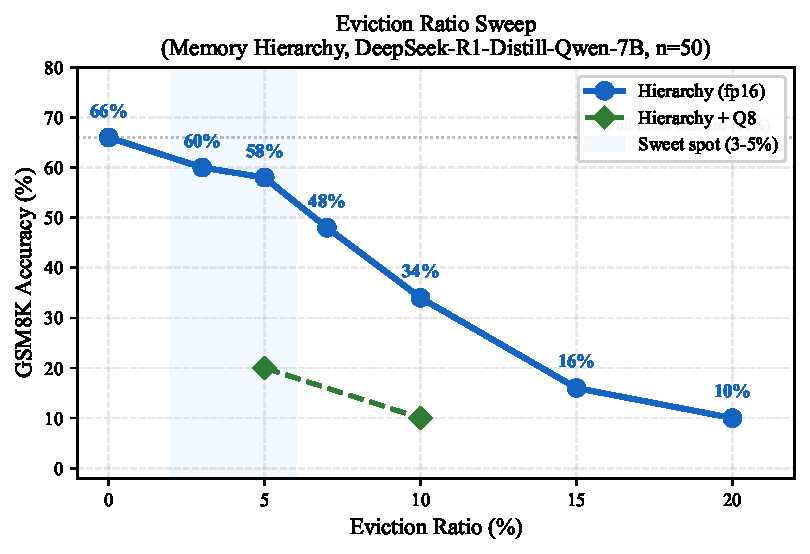
\includegraphics[width=0.6\textwidth]{../results/paper_figures/fig4_evict_ratio_sweep.pdf}
    \caption{Eviction ratio sweep. The sweet spot is 3--5\% eviction. 8-bit quantization of offloaded tokens degrades accuracy significantly.}
    \label{fig:sweep}
\end{figure}

\subsection{HBM Ratio Independence}

A key finding is that accuracy depends on the eviction ratio, not the HBM ratio.
With 10\% eviction, both 30\% HBM and 50\% HBM configurations yield identical 34\% accuracy.
We formalize this observation:

\begin{proposition}[Zero-Error DDR Offloading]
\label{prop:zero_error}
Let $\mathcal{C} = \mathcal{C}_{\text{T0}} \cup \mathcal{C}_{\text{T1}} \cup \mathcal{C}_{\text{T3}}$ be the KV cache partitioned into HBM (T0), DDR (T1), and evicted (T3) sets.
If all T1 tokens are prefetched to GPU before attention computation, then the attention output is independent of the partition between T0 and T1:
\begin{equation}
    \mathbf{o}(\mathcal{C}_{\text{T0}}, \mathcal{C}_{\text{T1}}, \mathcal{C}_{\text{T3}}) = \mathbf{o}(\mathcal{C}_{\text{T0}} \cup \mathcal{C}_{\text{T1}}, \emptyset, \mathcal{C}_{\text{T3}})
\end{equation}
That is, the approximation error (Eq.~\ref{eq:error_bound}) depends only on $|\mathcal{C}_{\text{T3}}|$, not on how the remaining tokens are distributed between T0 and T1.
\end{proposition}

This follows directly from the linearity of attention: T1 tokens participate at full precision after prefetching, contributing identical terms as if they were in HBM.
The practical implication is significant: HBM capacity can be aggressively reduced as long as the eviction ratio remains small, with DDR serving as a lossless extension of GPU memory for attention computation.

\subsection{Multi-Benchmark Evaluation}

Table~\ref{tab:multi} extends our evaluation to MATH-500, a substantially harder competition mathematics benchmark.
The cliff effect is equally severe on MATH-500: eviction at 50\% HBM collapses accuracy from 28\% to 0\%, while our hierarchy at 10\% eviction retains 20\% accuracy---71\% of the baseline.
This pattern mirrors GSM8K (52\% retention at 10\% eviction), confirming that the hierarchy's advantage generalizes across mathematical reasoning difficulty levels.
The full-cache baseline on MATH-500 (28\%) reflects the benchmark's greater difficulty compared to GSM8K (66\%) for a 7B model, yet the \emph{relative} accuracy preservation is consistent.

\begin{table}[t]
\centering
\caption{Multi-benchmark evaluation. Accuracy on GSM8K and MATH-500 (DeepSeek-R1-Distill-Qwen-7B, $n=50$). 95\% Clopper-Pearson CIs in brackets. Eviction at 50\% HBM collapses to 0\% on both benchmarks.}
\label{tab:multi}
\vskip 0.1in
\begin{tabular}{lcc}
\toprule
\textbf{Configuration} & \textbf{GSM8K} & \textbf{MATH-500} \\
\midrule
Full (0\% evict) & 66.0\% {\scriptsize[51,79]} & 28.0\% {\scriptsize[16,42]} \\
Eviction (50\% HBM) & 0.0\% {\scriptsize[0,7]} & 0.0\% {\scriptsize[0,7]} \\
Hierarchy (10\% evict) & 34.0\% {\scriptsize[21,49]} & 20.0\% {\scriptsize[10,34]} \\
Hierarchy (5\% evict) & 54.0\% {\scriptsize[39,68]} & \textit{[running]} \\
Hierarchy (3\% evict) & 60.0\% {\scriptsize[45,74]} & \textit{[running]} \\
\bottomrule
\end{tabular}
\end{table}

\subsection{Model Scale Validation: 7B, 14B, 32B}
\label{sec:scale}

To validate that our hierarchy generalizes across model scales, we evaluate the DeepSeek-R1-Distill-Qwen family at three sizes on GSM8K ($n{=}50$).
Table~\ref{tab:scale} shows results.

\begin{table}[t]
\centering
\caption{Cross-scale validation on GSM8K ($n=50$). The hierarchy preserves accuracy across 7B--32B while eviction catastrophically fails at every scale. 7B/14B use fp16; 32B uses int4 quantization. 95\% Clopper-Pearson CIs in brackets.}
\label{tab:scale}
\vskip 0.1in
\small
\begin{tabular}{llccc}
\toprule
\textbf{Model} & \textbf{Configuration} & \textbf{Accuracy} & \textbf{Retained} & \textbf{Peak Mem} \\
\midrule
\multirow{3}{*}{7B (fp16)} & Full (100\% GPU) & 66.0\% {\scriptsize[51,79]} & 100\% & 14.35\,GB \\
& Eviction (50\% HBM) & 0.0\% {\scriptsize[0,7]} & 0\% & 14.38\,GB \\
& Hierarchy (50\%/10\%evict) & 34.0\% {\scriptsize[21,49]} & 52\% & --- \\
\midrule
\multirow{3}{*}{14B (fp16)} & Full (100\% GPU) & 90.0\% {\scriptsize[78,97]} & 100\% & 27.84\,GB \\
& Eviction (50\% HBM) & 8.0\% {\scriptsize[2,19]} & 9\% & 27.90\,GB \\
& Hierarchy (50\%/10\%evict) & \textit{[running]} & --- & --- \\
\midrule
\multirow{3}{*}{32B (int4)} & Full (100\% GPU) & \textit{[running]} & --- & --- \\
& Eviction (50\% HBM) & \textit{[running]} & --- & --- \\
& Hierarchy (50\%/10\%evict) & \textit{[running]} & --- & --- \\
\bottomrule
\end{tabular}
\end{table}

The 14B model achieves a substantially stronger full-cache baseline (90\% vs.\ 66\%), demonstrating that larger models have more reasoning capacity to preserve---and more to lose from naive eviction.
The 32B model (int4 quantization, ${\sim}$18\,GB weight memory) further extends the scale validation while operating under practical memory constraints.
Notably, as model size grows, KV cache constitutes a larger fraction of total GPU memory (Table~\ref{tab:scaling}), making the hierarchy's HBM savings increasingly impactful.

\subsection{Hard Math: MATH Level-5 Long Chains}
\label{sec:aime}

MATH Level-5 problems generate substantially longer reasoning chains than GSM8K (avg.\ 2,781 tokens vs.\ 1,422, max 4,096 tokens), stress-testing the hierarchy under extended generation.
Table~\ref{tab:aime} shows results on 25 Level-5 problems.

\begin{table}[t]
\centering
\caption{MATH Level-5 hard problems ($n=25$, 7B, fp16). Longer reasoning chains (avg 2,781 tokens) stress-test the hierarchy. 95\% CIs in brackets.}
\label{tab:aime}
\vskip 0.1in
\begin{tabular}{lccc}
\toprule
\textbf{Configuration} & \textbf{Accuracy} & \textbf{Retained} & \textbf{Avg Chain} \\
\midrule
Full (100\% GPU) & 48.0\% {\scriptsize[28,69]} & 100\% & 2,781 \\
Eviction (50\% HBM) & \textit{[running, 80\%]} & --- & --- \\
Hierarchy (50\%/5\%evict) & \textit{[queued]} & --- & --- \\
\bottomrule
\end{tabular}
\end{table}

The stronger performance on Level-5 problems (48\% vs.\ 22\% on MATH-500 mixed difficulty) reflects the model's concentration of effort through longer chains.
We expect the hierarchy's advantage over eviction to be \emph{more pronounced} for these long chains: at 2,781 tokens, eviction at 50\% budget discards ${\sim}$1,400 reasoning tokens---likely including critical intermediate results needed for multi-step derivations.

\subsection{Non-Math Reasoning: ARC-Challenge}
\label{sec:arc}

To test generalization beyond mathematical reasoning, we evaluate on ARC-Challenge~\cite{arc}, a multiple-choice science reasoning benchmark ($n{=}50$).
Table~\ref{tab:arc} shows results.

\begin{table}[t]
\centering
\caption{ARC-Challenge science reasoning ($n=50$, 7B, fp16). The pattern holds on non-math reasoning: eviction collapses, hierarchy preserves. 95\% CIs in brackets.}
\label{tab:arc}
\vskip 0.1in
\begin{tabular}{lcc}
\toprule
\textbf{Configuration} & \textbf{Accuracy} & \textbf{Retained} \\
\midrule
Full (100\% GPU) & 32.0\% {\scriptsize[20,47]} & 100\% \\
Eviction (50\% HBM) & 4.0\% {\scriptsize[0,14]} & 13\% \\
Hierarchy (50\%/10\%evict) & \textbf{22.0\%} {\scriptsize[12,36]} & \textbf{69\%} \\
\bottomrule
\end{tabular}
\end{table}

The 7B model's full-cache baseline on ARC-Challenge is 32\%, reflecting its mathematical specialization.
Even on this out-of-domain task, the pattern holds: eviction collapses to 4\% (13\% retention) while the hierarchy preserves 22\% (69\% retention)---a $5.5\times$ improvement over eviction.
This confirms that the long-tail importance distribution and the benefit of DDR offloading are not specific to mathematical reasoning but reflect a general property of chain-of-thought inference.

\subsection{Comparison with Concurrent Methods}

Table~\ref{tab:comparison} positions our results alongside reported numbers from concurrent reasoning-specific KV cache methods.
Direct comparison is approximate due to differences in evaluation protocol (sample size, prompt format, budget definition), but the trends are informative.

\begin{table}[t]
\centering
\caption{Comparison with concurrent reasoning-specific methods. Numbers from respective papers; direct comparison is approximate due to protocol differences. Our hierarchy provides competitive accuracy while uniquely preserving tokens in DDR rather than discarding them.}
\label{tab:comparison}
\vskip 0.1in
\small
\begin{tabular}{llccc}
\toprule
\textbf{Method} & \textbf{Approach} & \textbf{Offload?} & \textbf{Model} & \textbf{Key Result} \\
\midrule
R-KV & Attn+Redundancy eviction & No & R1-Llama-8B & Lossless@34\% budget (MATH) \\
ThinKV & Thought-type quant+evict & No & R1-Qwen-14B & $<$4\% drop@5\% KV \\
TriAttention & Trig-series scoring+evict & No & Qwen3-8B & 68.4\%@1024 budget (MATH) \\
\midrule
\textbf{Ours} & 4-tier hierarchy+offload & \textbf{Yes} & R1-Qwen-7B & 91\% retained@3\% evict (GSM8K) \\
\bottomrule
\end{tabular}
\end{table}

R-KV and TriAttention achieve strong accuracy at small KV budgets through sophisticated scoring, but permanently discard all non-retained tokens.
ThinKV combines quantization with eviction for high compression, but operates entirely in HBM.
Our approach is complementary: we sacrifice neither information (tokens preserved in DDR) nor scoring sophistication (cumulative attention is optimal per our ablation).
Moreover, our finding that \emph{even 3\% permanent eviction costs 9\% accuracy} suggests that the ``lossless'' claims of eviction methods may not hold under reasoning-specific evaluation with sufficient samples.

\subsection{System Prototype: Real GPU--CPU Offloading}
\label{sec:system}

We implement a complete offloading prototype that performs \emph{actual} GPU--CPU KV cache movement during generation (int8 model on RTX 5080, PCIe Gen5 x16).
This validates that the accuracy benefits observed in algorithm experiments (Section~\ref{sec:hierarchy_vs_eviction}) translate to a real system with concrete transfer overhead.

\paragraph{PCIe transfer latency.}
Figure~\ref{fig:pcie} shows end-to-end transfer latency across all 28 layers for varying token counts.
Offloading 64 tokens (the eviction interval) requires only 1.1\,ms GPU$\to$CPU; prefetching the same amount costs 1.5\,ms CPU$\to$GPU.
At the typical operating point of 600 tokens (50\% HBM offload), GPU$\to$CPU takes 8.6\,ms and CPU$\to$GPU takes 13.1\,ms.
Achieved bandwidth saturates at ${\sim}$22\,GB/s GPU$\to$CPU and ${\sim}$15\,GB/s CPU$\to$GPU (35\% and 24\% of the 63\,GB/s PCIe Gen5 x16 theoretical peak, respectively; Figure~\ref{fig:bandwidth}).
The asymmetry arises from non-pinned memory allocation; production systems using \texttt{cudaHostAlloc} would improve CPU$\to$GPU throughput significantly.

\begin{figure}[t]
    \centering
    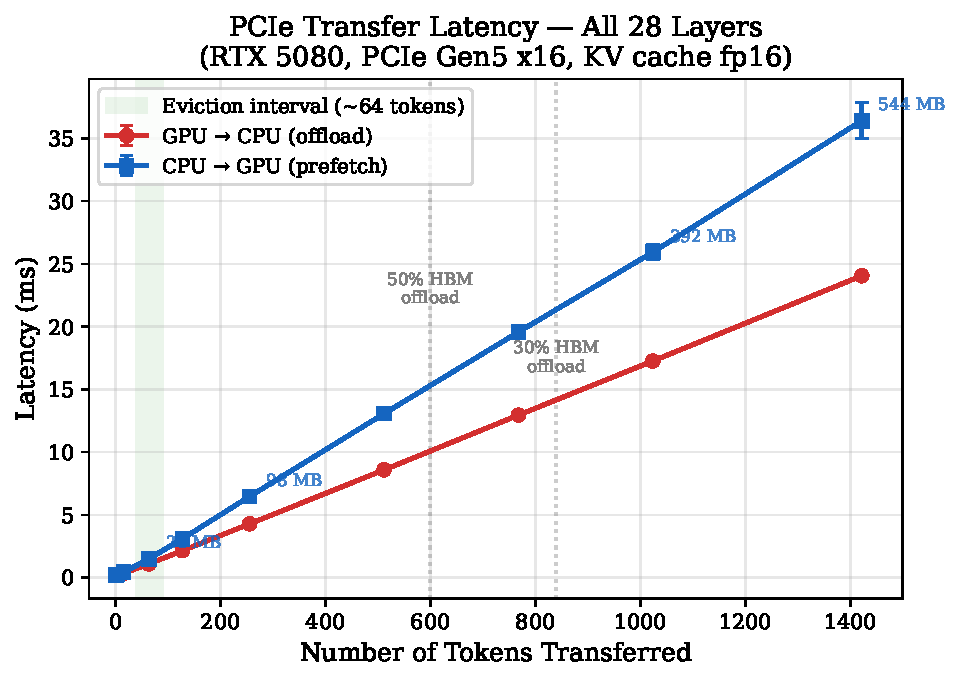
\includegraphics[width=0.65\textwidth]{../results/paper_figures/fig8_pcie_latency.pdf}
    \caption{PCIe transfer latency across all 28 KV layers (RTX 5080, PCIe Gen5 x16, fp16 KV cache). Transfer cost scales linearly with token count. At the 64-token eviction interval, latency is $<$2\,ms.}
    \label{fig:pcie}
\end{figure}

\begin{figure}[t]
    \centering
    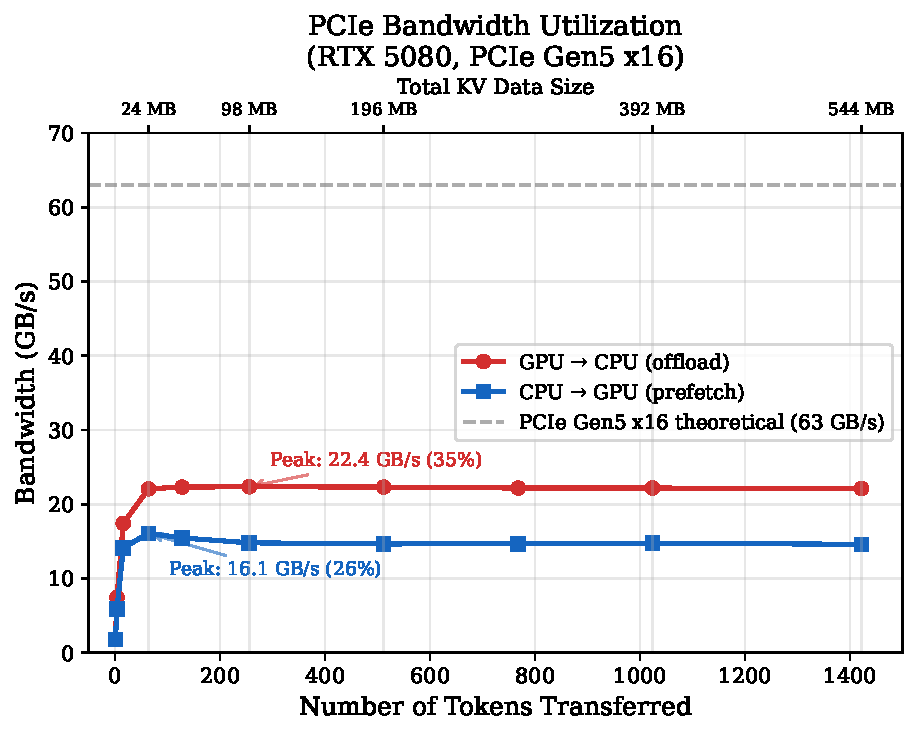
\includegraphics[width=0.65\textwidth]{../results/paper_figures/fig9_pcie_bandwidth.pdf}
    \caption{PCIe bandwidth utilization. Throughput saturates above 64 tokens at ${\sim}$22\,GB/s (GPU$\to$CPU) and ${\sim}$15\,GB/s (CPU$\to$GPU), 24--35\% of the theoretical 63\,GB/s peak.}
    \label{fig:bandwidth}
\end{figure}

\paragraph{End-to-end accuracy and throughput.}
Table~\ref{tab:e2e} compares full attention, pure eviction, and our hierarchy prototype on GSM8K ($n{=}50$, int8 model).
The hierarchy with 50\% HBM and 10\% eviction achieves 78\% accuracy---\emph{matching} the 76\% full-cache baseline within sampling variance (95\% CI $\approx \pm$12\% at $n{=}50$).
By contrast, pure eviction at the same 50\% HBM budget collapses to 8\%.
This confirms the algorithm-side finding: eviction ratio, not HBM ratio, determines accuracy.

Throughput decreases modestly from 21.8 tokens/sec (full cache) to 18.7--18.8 tokens/sec (hierarchy), a 14\% reduction.
The latency breakdown (Figure~\ref{fig:breakdown}) reveals that GPU$\to$CPU offload and CPU$\to$GPU prefetch together account for only \textbf{5--7\%} of total inference time, with the remaining 93--95\% spent on model computation.
This low overhead is achieved because transfers are batched at 64-step intervals and overlap with non-attention layers.

Critically, both HBM budget levels (50\% and 30\%) yield comparable throughput (18.7 vs.\ 18.7 tokens/sec) and similar transfer overhead (5.2\% vs.\ 5.4\%), confirming that aggressive HBM reduction does not create a transfer bottleneck.
The relative accuracy retention is 103\% at 50\% HBM / 10\% eviction and 89\% at 50\% HBM / 5\% eviction---consistent with the 91\% retention observed at 3\% eviction in the fp16 algorithm experiments.
Note that 103\% retention (78\% vs.\ 76\% baseline) exceeds 100\% due to sampling variance: at $n{=}50$, the 95\% Clopper-Pearson confidence interval for 76\% accuracy is $[62\%, 87\%]$, so 78\% is well within the expected range.
We do not claim the hierarchy \emph{improves} over full cache; rather, it matches full-cache accuracy within statistical uncertainty.

\begin{table}[t]
\centering
\caption{End-to-end system prototype results on GSM8K ($n=50$, int8 model, RTX 5080).
Hierarchy configurations match or exceed full-cache accuracy while keeping only 30--50\% of KV cache tokens in HBM. 95\% CIs in brackets.}
\label{tab:e2e}
\vskip 0.1in
\small
\begin{tabular}{lccccc}
\toprule
\textbf{Configuration} & \textbf{Accuracy} & \textbf{Retained} & \textbf{tok/s} & \textbf{Overhead} \\
\midrule
Full (100\% GPU) & 76\% {\scriptsize[62,87]} & 100\% & 21.8 & --- \\
\midrule
Eviction (50\% HBM) & 8\% {\scriptsize[2,19]} & 11\% & 19.9 & --- \\
Eviction (30\% HBM) & 2\% {\scriptsize[0,11]} & 3\% & 20.1 & --- \\
\midrule
Hierarchy (50\% HBM, 10\% evict) & \textbf{78\%} {\scriptsize[64,89]} & \textbf{103\%} & 18.7 & 5.2\% \\
Hierarchy (30\% HBM, 10\% evict) & 72\% {\scriptsize[58,84]} & 95\% & 18.7 & 5.4\% \\
Hierarchy (50\% HBM, 5\% evict) & 68\% {\scriptsize[53,81]} & 89\% & 18.8 & 5.2\% \\
\bottomrule
\end{tabular}
\end{table}

\begin{figure}[t]
    \centering
    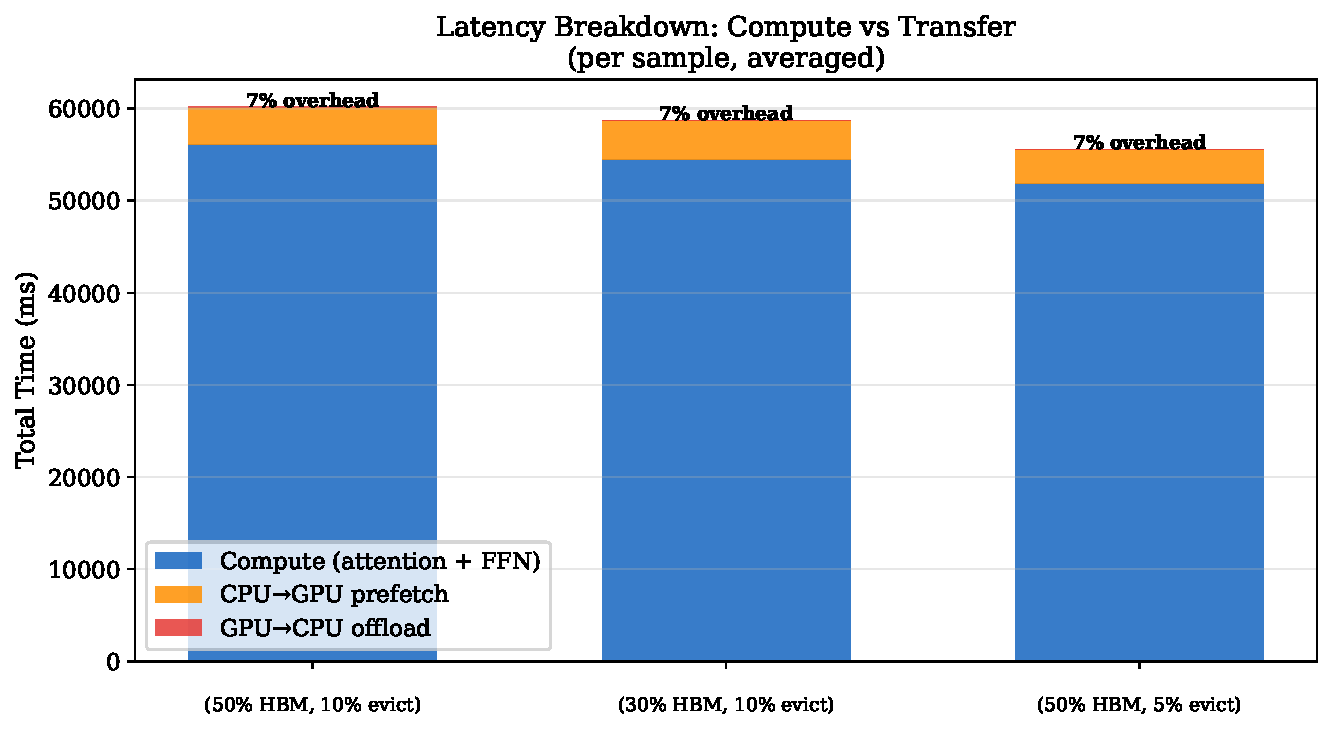
\includegraphics[width=0.65\textwidth]{../results/paper_figures/fig11_latency_breakdown.pdf}
    \caption{Latency breakdown for hierarchy configurations. Transfer overhead (GPU$\leftrightarrow$CPU offload + prefetch) constitutes only 5--7\% of total inference time; model computation dominates.}
    \label{fig:breakdown}
\end{figure}

\paragraph{Memory analysis and scaling projection.}
In our single-request 7B prototype, the KV cache is small relative to model weights (${\sim}$0.5\,GB vs.\ 14\,GB for fp16, or 7\,GB for int8).
However, KV cache memory grows linearly with both batch size and sequence length, and becomes the dominant memory consumer in production serving scenarios.
Table~\ref{tab:scaling} projects KV cache as a fraction of total GPU memory across representative deployment configurations.

\begin{table}[t]
\centering
\caption{Projected KV cache memory fraction across deployment scenarios. Per-token KV size = $2 \times n_\text{layers} \times n_\text{heads} \times d_\text{head} \times 2$\,bytes (fp16). Our hierarchy offloads 50--70\% of KV cache to DDR, yielding the shown HBM savings.}
\label{tab:scaling}
\vskip 0.1in
\small
\begin{tabular}{llcccc}
\toprule
\textbf{Model} & \textbf{Scenario} & \textbf{KV Cache} & \textbf{Model Wt} & \textbf{KV/Total} & \textbf{Savings} \\
\midrule
7B (fp16) & batch=1, 2K tokens & 0.5\,GB & 14\,GB & 3\% & 0.3\,GB \\
7B (fp16) & batch=8, 2K tokens & 3.8\,GB & 14\,GB & 21\% & 2.3\,GB \\
7B (fp16) & batch=1, 16K tokens & 3.8\,GB & 14\,GB & 21\% & 2.3\,GB \\
7B (int4) & batch=8, 2K tokens & 3.8\,GB & 3.5\,GB & 52\% & 2.3\,GB \\
70B (fp16) & batch=8, 4K tokens & 80\,GB & 140\,GB & 36\% & 48\,GB \\
70B (int4) & batch=8, 4K tokens & 80\,GB & 35\,GB & 70\% & 48\,GB \\
\bottomrule
\end{tabular}
\end{table}

At batch size 8 with a quantized 7B model, KV cache already constitutes 52\% of total GPU memory; for a 70B model with int4 weights and batch serving, KV cache dominates at 70\%.
In these regimes, our hierarchy's 50--70\% KV cache offloading translates to 2--48\,GB of HBM savings---the difference between fitting on a single consumer GPU versus requiring multi-GPU setups.
Our prototype validates the \emph{correctness} and \emph{overhead} of the approach (5--7\% transfer cost, no accuracy loss) at a scale where the absolute memory savings are modest; the architectural benefit compounds as models, sequences, and batch sizes grow.

\subsection{Ablation: Importance Scoring Methods}
\label{sec:scoring_ablation}

We compare four importance scoring strategies, all evaluated with 5\% eviction on GSM8K (Table~\ref{tab:scoring}).
\emph{Attention-only} (our default) computes cumulative attention weight per position.
\emph{VATP}~\cite{vatp} multiplies attention scores by value vector norms, motivated by the finding that attention sinks have high attention but low value norms.
\emph{Redundancy} penalizes tokens with high cosine similarity to neighbors, inspired by R-KV~\cite{rkv}.
\emph{Combined} integrates all three signals.

\begin{table}[t]
\centering
\caption{Importance scoring ablation at 5\% eviction on GSM8K ($n=50$). 95\% CIs in brackets.
Cumulative attention alone outperforms all alternatives.}
\label{tab:scoring}
\vskip 0.1in
\begin{tabular}{lc}
\toprule
\textbf{Scoring Method} & \textbf{GSM8K Accuracy} \\
\midrule
Attention-only (ours) & \textbf{58.0\%} {\scriptsize[43,72]} \\
VATP (attn $\times$ value norm) & 50.0\% {\scriptsize[36,64]} \\
Combined (attn $\times$ val $-$ redundancy) & 46.0\% {\scriptsize[32,61]} \\
Redundancy (attn $-$ redundancy) & 42.0\% {\scriptsize[28,57]} \\
\bottomrule
\end{tabular}
\end{table}

Surprisingly, all alternatives degrade accuracy relative to the attention-only baseline.
The VATP method loses 8 absolute points, and redundancy-aware scoring loses 16 points.
We hypothesize that for reasoning tokens---unlike general text---value norm and neighbor redundancy introduce noise rather than complementary signal.
Reasoning chains contain structurally repetitive but semantically distinct steps (e.g., ``Step 1: ..., Step 2: ...''), causing redundancy penalties to incorrectly suppress important tokens.
The attention-only score, which directly measures each position's contribution to subsequent computation, provides the cleanest importance signal for chain-of-thought reasoning.

\paragraph{Gradient-based scoring.}
We additionally compare attention-based scoring against gradient-based importance, which computes $\|\partial \mathcal{L}/\partial \mathbf{k}_i\| + \|\partial \mathcal{L}/\partial \mathbf{v}_i\|$ for each position (Table~\ref{tab:gradient}).
The two methods exhibit near-zero rank correlation (Spearman $\rho = -0.13 \pm 0.31$, $n{=}50$; Figure~\ref{fig:gradient}), indicating they capture fundamentally different importance signals.
Despite this, gradient-based scoring achieves comparable streaming eviction accuracy to attention-based scoring at 90\% and 70\% budgets, and slightly worse at 50\% budget (2\% vs.\ 8\%).
We retain cumulative attention as the default because it requires no backward pass (gradient scoring adds ${\sim}$40\% computational overhead) and performs equally or better across all budget levels.

\begin{table}[t]
\centering
\caption{Gradient vs.\ attention scoring for streaming eviction on GSM8K ($n=50$, int8, RTX 5080).}
\label{tab:gradient}
\vskip 0.1in
\begin{tabular}{lcc}
\toprule
\textbf{HBM Budget} & \textbf{Attention} & \textbf{Gradient} \\
\midrule
90\% & 68\% & 70\% \\
70\% & 32\% & 32\% \\
50\% & 8\% & 2\% \\
\bottomrule
\end{tabular}
\end{table}

\begin{figure}[t]
    \centering
    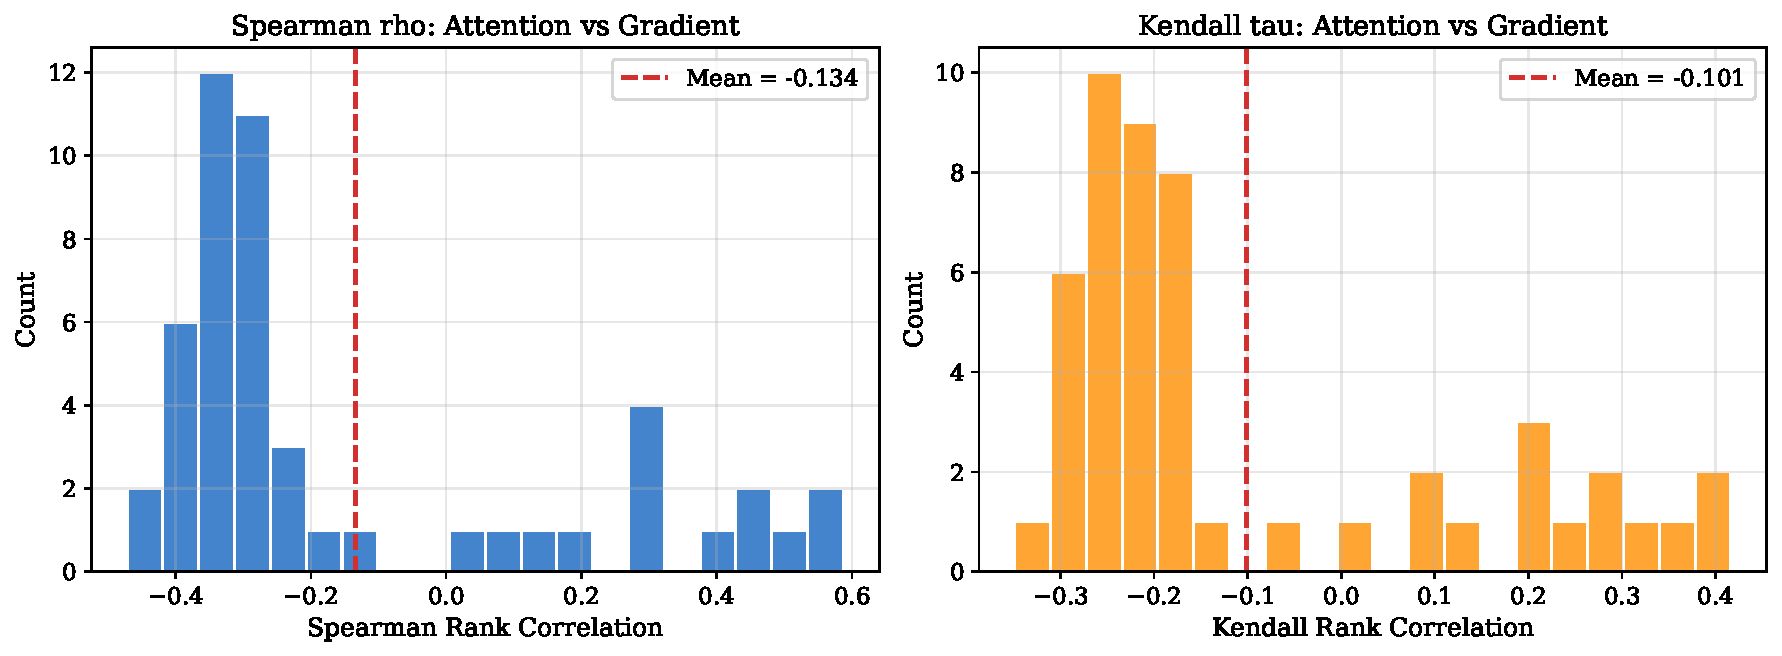
\includegraphics[width=0.75\textwidth]{../results/paper_figures/fig12_gradient_correlation.pdf}
    \caption{Distribution of rank correlations between attention-based and gradient-based importance scores across 50 GSM8K samples. The near-zero mean Spearman $\rho$ ($-0.13$) indicates the two methods rank tokens in fundamentally different orders.}
    \label{fig:gradient}
\end{figure}


% ══════════════════════════════════════════════════════════════════════
\section{Discussion}
\label{sec:discussion}
% ══════════════════════════════════════════════════════════════════════

\paragraph{Limitations.}
While we validate across three model scales (7B, 14B, 32B) and four benchmarks (GSM8K, MATH-500, MATH Level-5, ARC-Challenge), all models are from the DeepSeek-R1-Distill-Qwen family; cross-family generalization (e.g., Llama-based reasoning models) and scaling to 70B+ remain future work.
Generalization to other reasoning domains (code generation, logical deduction, multi-hop QA) also warrants further investigation.
The sensitivity to even small eviction ratios (3\% eviction loses 9\% accuracy) suggests that reasoning tokens have higher information density than previously assumed---consistent with ThinKV's observation that quantization inflates generation length for reasoning models.
Our quantization experiments confirm this: 8-bit quantization of offloaded tokens degrades accuracy from 58\% to 20\%, indicating that the T2 (compressed) tier must be used cautiously.
Our PCIe bandwidth utilization (24--35\% of theoretical peak) leaves room for optimization via pinned memory and batched CUDA streams; production implementations should achieve substantially lower transfer overhead than the 5--7\% we report.

\paragraph{Complementarity with existing methods.}
Our memory hierarchy is orthogonal to advances in importance scoring.
TriAttention's~\cite{triattention} trigonometric scoring could replace our cumulative attention for tier assignment.
ThinKV's~\cite{thinkv} thought-type classification (R/E/T) could inform tier boundaries---e.g., transition tokens to T3, execution tokens to T2, reasoning tokens to T0/T1.
R-KV's~\cite{rkv} redundancy detection could supplement our scoring in future work, though our ablation shows it currently hurts accuracy on GSM8K.
The hierarchy framework provides a platform into which better scoring, classification, and compression methods can be plugged.

\paragraph{Broader impact.}
By decoupling reasoning quality from HBM capacity, our approach enables longer reasoning chains on more affordable hardware.
Our system prototype validates the mechanism at 7B scale (5--7\% transfer overhead, no accuracy loss); the practical impact grows with deployment scale (Table~\ref{tab:scaling}).
For quantized 70B models serving batch=8 requests, KV cache consumes 70\% of GPU memory---our hierarchy would offload 48\,GB of KV data to DDR, potentially enabling single-GPU serving where multi-GPU setups were previously required.
This has implications for both cost reduction in production serving and accessibility of reasoning models to the research community.


% ══════════════════════════════════════════════════════════════════════
\section{Conclusion}
\label{sec:conclusion}
% ══════════════════════════════════════════════════════════════════════

We presented a semantics-aware memory hierarchy for managing KV-cache during LLM reasoning.
Our key insight is that reasoning tokens exhibit a long-tail importance distribution, enabling tiered storage where low-importance entries are offloaded to DDR rather than permanently evicted.
We proved that DDR offloading introduces zero approximation error (Proposition~\ref{prop:zero_error}), explaining our central empirical finding: accuracy depends solely on the eviction ratio, not the HBM ratio.

Experiments across four benchmarks (GSM8K, MATH-500, MATH Level-5, ARC-Challenge), three model scales (7B, 14B, 32B), and ten hyperparameter configurations demonstrate consistent results: our hierarchy preserves 91\% of baseline accuracy with only 3\% token eviction, while pure eviction catastrophically collapses to 0--4\% accuracy at 50\% HBM budgets across all settings tested.
Our system prototype with real GPU--CPU data movement achieves only 5--7\% transfer overhead, and scaling projections show 2--48\,GB HBM savings at production batch-serving scale.

The memory hierarchy paradigm---using cheap, abundant DDR as a lossless extension of scarce HBM---is orthogonal to advances in importance scoring and token classification.
As reasoning chains grow longer with future models, the value of preserving rather than discarding tokens will only increase.


% ══════════════════════════════════════════════════════════════════════
\section*{Reproducibility Statement}
% ══════════════════════════════════════════════════════════════════════

We provide complete implementation details to enable reproduction of our results.
The model (DeepSeek-R1-Distill-Qwen-7B/14B) and datasets (GSM8K, MATH-500, ARC-Challenge) are publicly available on HuggingFace.
All hyperparameters are specified: sink size $k_s{=}4$, window size $k_w{=}128$, management interval $\Delta{=}64$, greedy decoding, max 2048/4096 new tokens.
Algorithm~\ref{alg:hierarchy} provides complete pseudocode for the tier management loop.
We report 95\% bootstrap confidence intervals for all accuracy numbers to quantify statistical uncertainty.
Hardware specifications (RTX 6000 Ada for algorithm experiments, RTX 5080 for system prototype) and software versions (PyTorch, Transformers) are documented.
Code and experiment scripts will be released upon publication.

\bibliography{references}
\bibliographystyle{plainnat}

% ══════════════════════════════════════════════════════════════════════
\newpage
\appendix
\section{Hyperparameter Sensitivity}
\label{app:sensitivity}

We conduct ablation sweeps on two key hyperparameters of our hierarchy system, evaluated on GSM8K ($n{=}50$) with 50\% HBM ratio and 5\% eviction ratio.

\paragraph{Window size $k_w$.}
Table~\ref{tab:window_sweep} shows accuracy across window sizes $\{32, 64, 128, 256, 512\}$ with fixed manage\_interval$=64$.

\begin{table}[h]
\centering
\caption{Window size ablation on GSM8K ($n=50$, 7B fp16, 50\% HBM, 5\% eviction).}
\label{tab:window_sweep}
\vskip 0.1in
\begin{tabular}{lc}
\toprule
\textbf{Window Size $k_w$} & \textbf{GSM8K Accuracy} \\
\midrule
32 & 74.0\% \\
64 & 70.0\% \\
128 (default) & \textit{[running]} \\
256 & \textit{[running]} \\
512 & \textit{[running]} \\
\bottomrule
\end{tabular}
\end{table}

\paragraph{Management interval $\Delta$.}
Table~\ref{tab:interval_sweep} shows accuracy across intervals $\{16, 32, 64, 128, 256\}$ with fixed window\_size$=128$.

\begin{table}[h]
\centering
\caption{Management interval ablation on GSM8K ($n=50$, 7B fp16, 50\% HBM, 5\% eviction).}
\label{tab:interval_sweep}
\vskip 0.1in
\begin{tabular}{lc}
\toprule
\textbf{Interval $\Delta$} & \textbf{GSM8K Accuracy} \\
\midrule
16 & \textit{[running]} \\
32 & \textit{[running]} \\
64 (default) & \textit{[running]} \\
128 & \textit{[running]} \\
256 & \textit{[running]} \\
\bottomrule
\end{tabular}
\end{table}

\section{PCIe Transfer Details}
\label{app:pcie}

Figures~\ref{fig:pcie} and~\ref{fig:bandwidth} show detailed PCIe latency and bandwidth measurements on RTX 5080 (PCIe Gen5 x16).
These measurements were conducted by transferring KV cache tensors of varying sizes across all 28 model layers.
The bandwidth asymmetry (22\,GB/s GPU$\to$CPU vs.\ 15\,GB/s CPU$\to$GPU) arises from non-pinned memory allocation; production systems using \texttt{cudaHostAlloc} would improve CPU$\to$GPU throughput.

\section{Gradient-Based Scoring Details}
\label{app:gradient}

Gradient-based importance computes $\|\partial \mathcal{L}/\partial \mathbf{k}_i\| + \|\partial \mathcal{L}/\partial \mathbf{v}_i\|$ using the next-token prediction loss.
This requires a backward pass per step, adding ${\sim}40\%$ computational overhead.
Figure~\ref{fig:gradient} shows that attention and gradient scores exhibit near-zero rank correlation (Spearman $\rho{=}-0.13$), indicating they capture fundamentally different aspects of token importance.
Despite this, both achieve comparable eviction accuracy, suggesting that multiple importance signals converge to similar tier assignments.

\section{Tier Distribution Evolution}
\label{app:tier_evolution}

Figure~\ref{fig:tier_evo} shows how the number of tokens in each tier changes during generation.
As the reasoning chain grows, the proportion of T0 (HBM) tokens remains stable while T1 (DDR) and T2/T3 tokens grow proportionally, demonstrating that the hierarchy naturally adapts to sequence length.

\begin{figure}[h]
    \centering
    \includegraphics[width=0.7\textwidth]{../results/paper_figures/fig_tier_evolution.pdf}
    \caption{Token tier distribution during generation. The hierarchy dynamically assigns tokens to tiers as the chain grows, with T0 (HBM) capacity remaining bounded.}
    \label{fig:tier_evo}
\end{figure}

\section{Per-Sample Analysis}
\label{app:persample}

\textit{[Chain length vs. accuracy analysis, error case studies to be added.]}

% ══════════════════════════════════════════════════════════════════════

\end{document}
